% Required preamble packages: \usepackage{graphicx,booktabs,subcaption}
% Figure paths assume the three verified PNG files are placed under images/.
\subsection{Empirical Motivation from Observed SSH Interactions}
\label{sec:empirical_motivation}

We examine SSH interaction records from a distributed honeypot deployment to
motivate two requirements of the proposed execution model: consistency with
accumulated session state and selective, evidence-supported response
adaptation. The session-linked subset spans 2 January--28 August 2025 and
contains 378,867 recorded events associated with 387 distinct session
identifiers in the distributed collection. Details that identify the
collection infrastructure are withheld for operational security.
Each event is a logging record linked to a session, not necessarily an
attacker command. 

To distinguish recorded activity from interpretable commands, we matched
captured input strings against 116 command-matching rules in the command
reference database and replaced recognized commands with their command IDs
(CIDs). Among session-linked records, 627 events are mapped to 53 distinct
CIDs, appearing in 339 sessions; the remaining 378,240 records are unmatched.
The latter are labeled \texttt{SCAN} in the processed dataset solely as a
processing category; this label does not establish that the records are
network scans. The resulting analysis units are
\begin{equation}
\begin{aligned}
N_{\mathrm{sess}} &= 387, &
N_{\mathrm{mapped\,sess}} &= 339,\\
N_{\mathrm{events}} &= 378{,}867, &
N_{\mathrm{CID\,events}} &= 627.
\end{aligned}
\label{eq:dataset_filtering}
\end{equation}
There are 48 additional retained sessions containing only unmatched
records. The source file also contains 463 events without a session ID;
these are excluded from session-level analyses. The available fields do
not permit reliable reconstruction of the number of SSH connection attempts
or sessions reaching a particular authentication stage, and we therefore
do not report such counts. Table~\ref{tab:ssh_summary} summarizes the
validated subset.

\begin{table}[!htbp]
\centering
\scriptsize
\caption{Verified SSH interaction subset used for empirical motivation.}
\label{tab:ssh_summary}
\begin{tabular}{lr}
\toprule
\textbf{Property} & \textbf{Value} \\
\midrule
Observation period & 2 Jan.--28 Aug. 2025 \\
Session-linked events & 378,867 \\
Recorded sessions (distinct session IDs) & 387 \\
Sessions containing $\geq 1$ mapped CID & 339 \\
Sessions containing only unmatched events & 48 \\
Mapped command events & 627 \\
Unmatched events (processing label \texttt{SCAN}) & 378,240 \\
Distinct mapped CIDs & 53 \\
Median recorded events per session & 1 \\
Single-event sessions & 230 (59.4\%) \\
Sessions with $\leq 2$ recorded events & 253 (65.4\%) \\
Sessions with $\leq 5$ recorded events & 288 (74.4\%) \\
\bottomrule
\end{tabular}
\end{table}

Recorded interaction depth is highly skewed
(Fig.~\ref{fig:ssh_empirical_motivation}a). The median is one event,
59.4\% of sessions contain one recorded event, and 74.4\% contain at most
five events. A small upper tail accounts for much of the aggregate record
volume; the largest session contains 10,940 records. However, almost all
session-linked records are unmatched by the command reference. Thus,
recorded-event depth does not measure the number of interpretable attacker
commands and must not be equated with the executed interaction steps used
to compute experimental episode-path length (EPL).

We next assess whether interpretable input continues after representative
command classes. For a session containing a mapped command from class
$g$, we define \emph{observable continuation} as at least one further
mapped command with a timestamp strictly later than the earliest mapped
occurrence of $g$ in that session. This rule avoids inferring within-second
ordering from the available one-second timestamp resolution. Command
classes are fixed sets of CIDs (specified in the analysis mapping); a
session may contribute to more than one class. Groups with fewer than
10 relevant sessions are omitted from the visualization. As shown in
Fig.~\ref{fig:ssh_empirical_motivation}b, timestamp-resolved continuation
is observed in 37 of 50 sessions containing shell/CLI probes (74.0\%) and
33 of 57 containing filesystem, navigation, or write-related commands
(57.9\%). The corresponding proportions are 6 of 21 (28.6\%) for payload
retrieval or staging, 3 of 15 (20.0\%) for network/device probing, and
24 of 243 (9.9\%) for architecture/binary checks. These quantities are
conservative with respect to same-second continuations and describe
observed association with subsequent mapped input, not a response-induced
behavioral effect. Differences in session context, action order, and
observation opportunity also preclude a causal interpretation.

Repeated capability checks provide a complementary reason to maintain
session-state consistency. We distinguish a \emph{repeated CID}, which
occurs at least twice in a session, from \emph{timestamp-resolved
revalidation}, in which the same CID is observed at times $t_1<t_3$
with a different mapped CID at an intermediate time $t_2$,
$t_1<t_2<t_3$. Under the first definition,
\texttt{sh} (CID~4) repeats in 25 of 44 relevant sessions (56.8\%),
\texttt{linuxshell} (CID~5) in 13 of 33 (39.4\%), and
binary inspection (CID~1) in 28 of 107 (26.2\%). The stricter
revalidation criterion is satisfied in 5 of 44 (11.4\%), 1 of 33
(3.0\%), and 2 of 107 (1.9\%) sessions, respectively
(Fig.~\ref{fig:ssh_empirical_motivation}c). These smaller counts reflect
what the available timestamp precision can establish unambiguously;
additional same-second action order cannot be recovered from this CSV.

Table~\ref{tab:observed_sequences} provides two sequences verified from
the captured data. Trace~A contains successive architecture inspection,
payload retrieval attempts, permission modification, file removal,
log modification, and session exit. The trace does not establish that a
payload was actually executed. Trace~B shows a shell probe, intervening
binary inspection, and a later recurrence of the shell probe at three
distinct timestamps. Both illustrate why a simulated property exposed
earlier in a session may need to remain consistent when queried again.

\begin{table*}[!htbp]
\centering
\scriptsize
\caption{Verified examples of temporally ordered mapped SSH inputs.
CIDs are the command IDs assigned using the supplied reference database.}
\label{tab:observed_sequences}
\begin{tabular}{p{0.7cm}p{8.8cm}p{6.8cm}}
\toprule
\textbf{Trace} & \textbf{Observed CID progression} & \textbf{Interpretation} \\
\midrule
A &
\texttt{CID72 $\rightarrow$ CID103 $\rightarrow$ CID94 $\rightarrow$ CID109
$\rightarrow$ CID110 $\rightarrow$ CID102 $\rightarrow$ CID17} &
Architecture check $\rightarrow$ retrieval attempts $\rightarrow$
permission change $\rightarrow$ file removal $\rightarrow$
log modification $\rightarrow$ exit \\
\addlinespace
B &
\texttt{CID4 $\rightarrow$ CID1 $\rightarrow$ CID4} &
Shell validation $\rightarrow$ binary inspection $\rightarrow$
subsequent shell revalidation \\
\bottomrule
\end{tabular}
\end{table*}

\begin{figure*}[!htbp]
\centering
\begin{subfigure}[t]{0.48\textwidth}
 \centering
 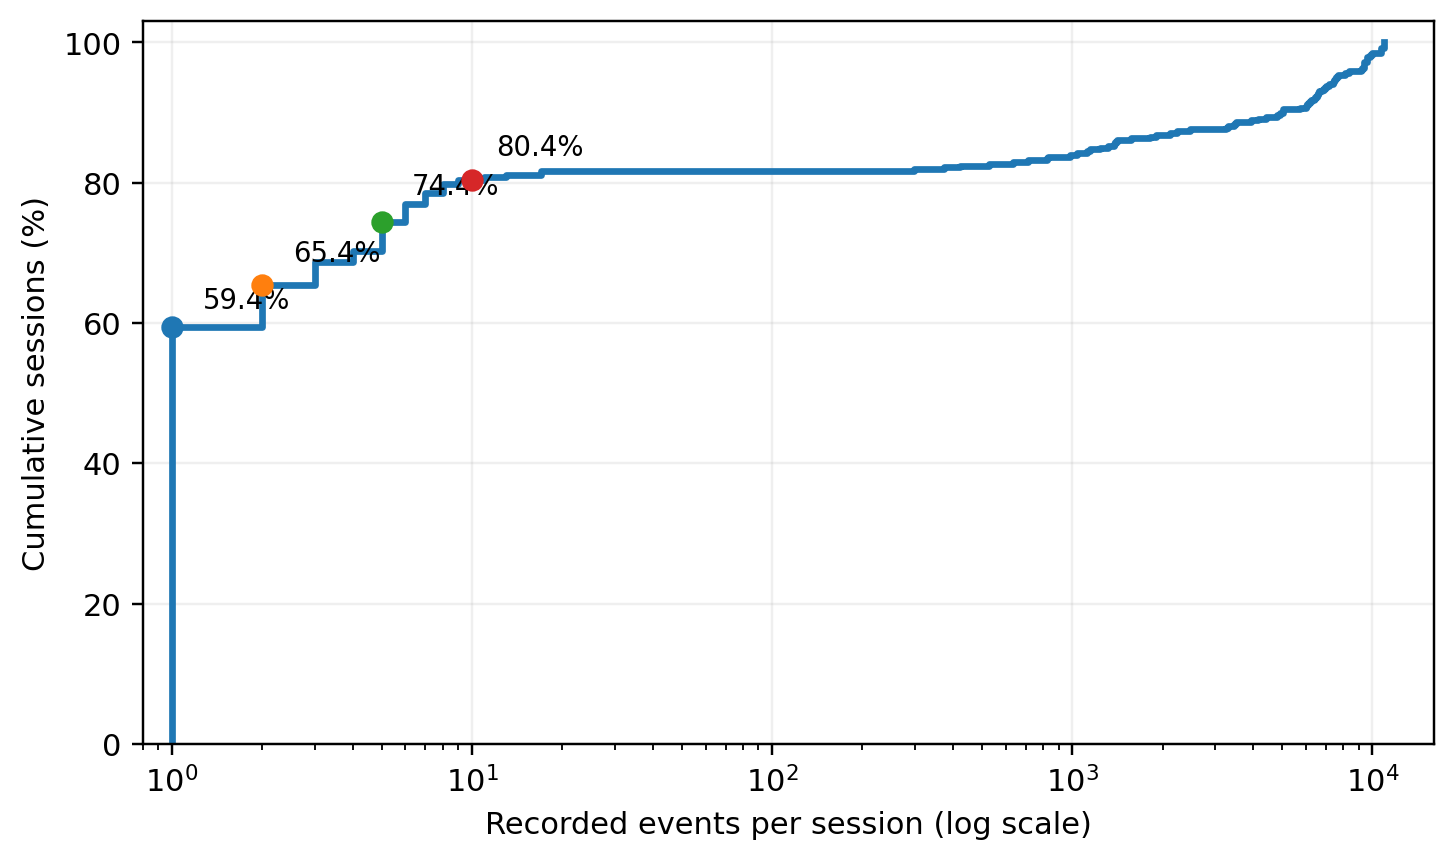
\includegraphics[width=\linewidth]{images/fig_empirical_session_depth_verified.png}
 \caption{Recorded-event depth per session (ECDF).}
\end{subfigure}
\hfill
\begin{subfigure}[t]{0.48\textwidth}
 \centering
 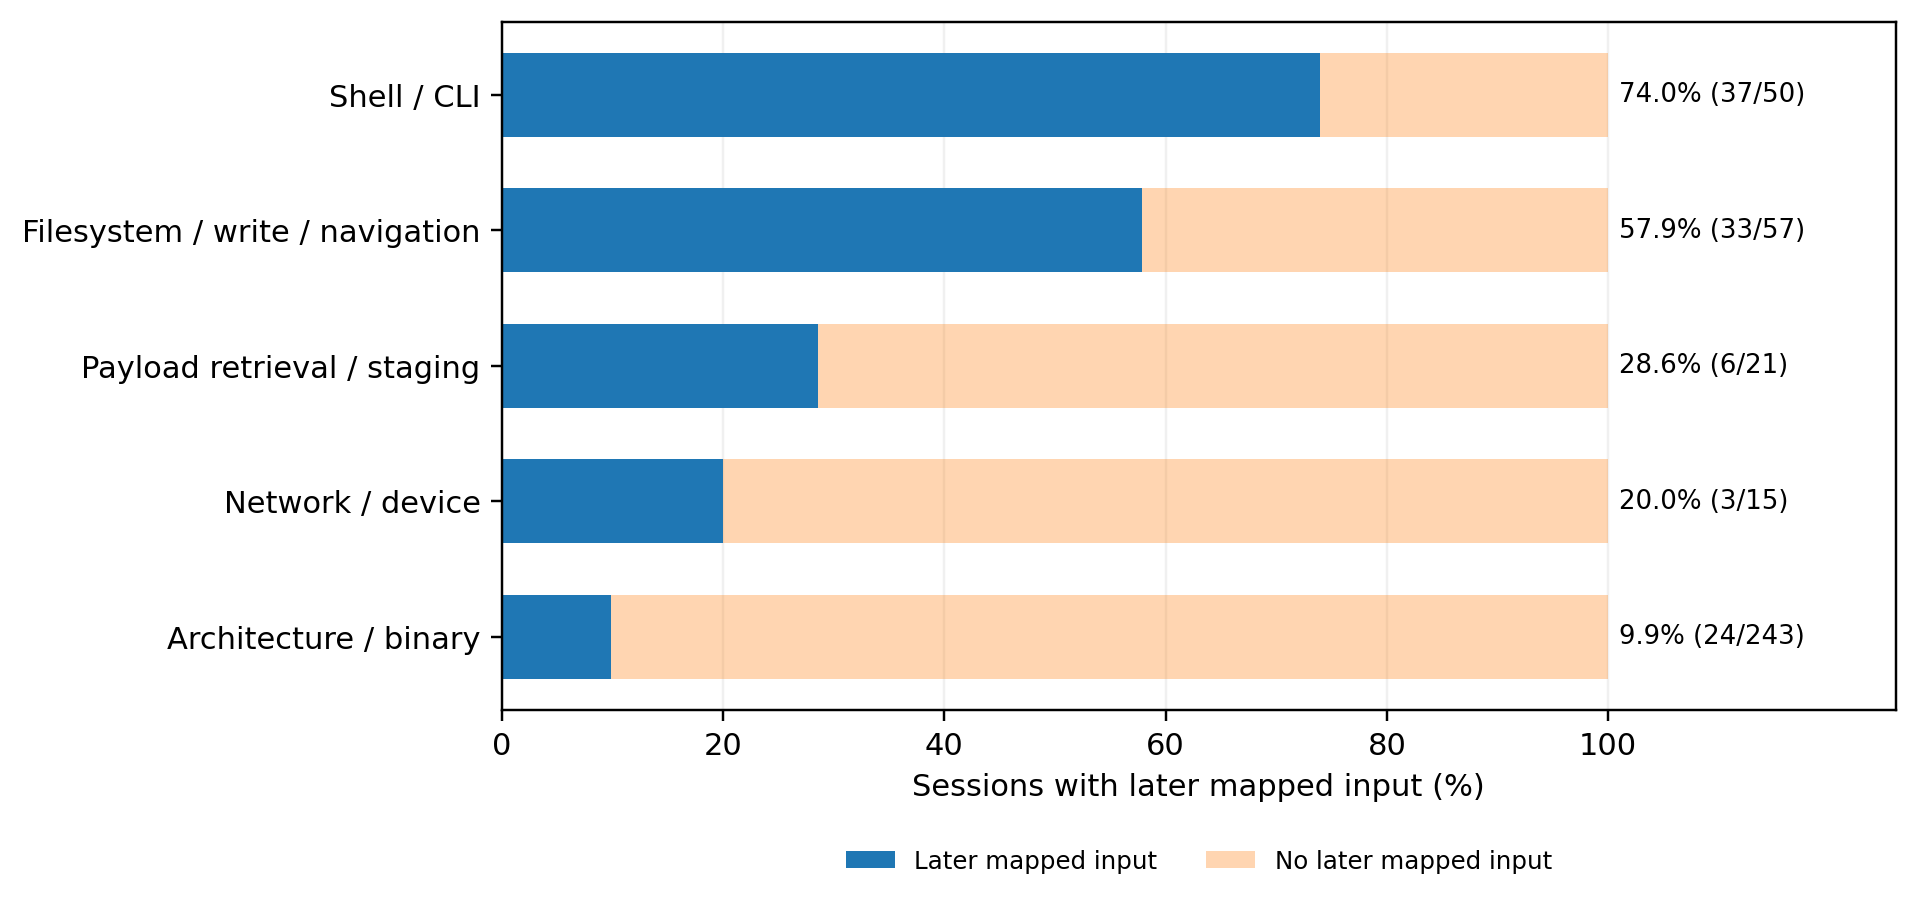
\includegraphics[width=\linewidth]{images/fig_probe_continuation_verified.png}
 \caption{Mapped-input continuation after probe classes.}
\end{subfigure}
\par\medskip
\begin{subfigure}[t]{0.67\textwidth}
 \centering
 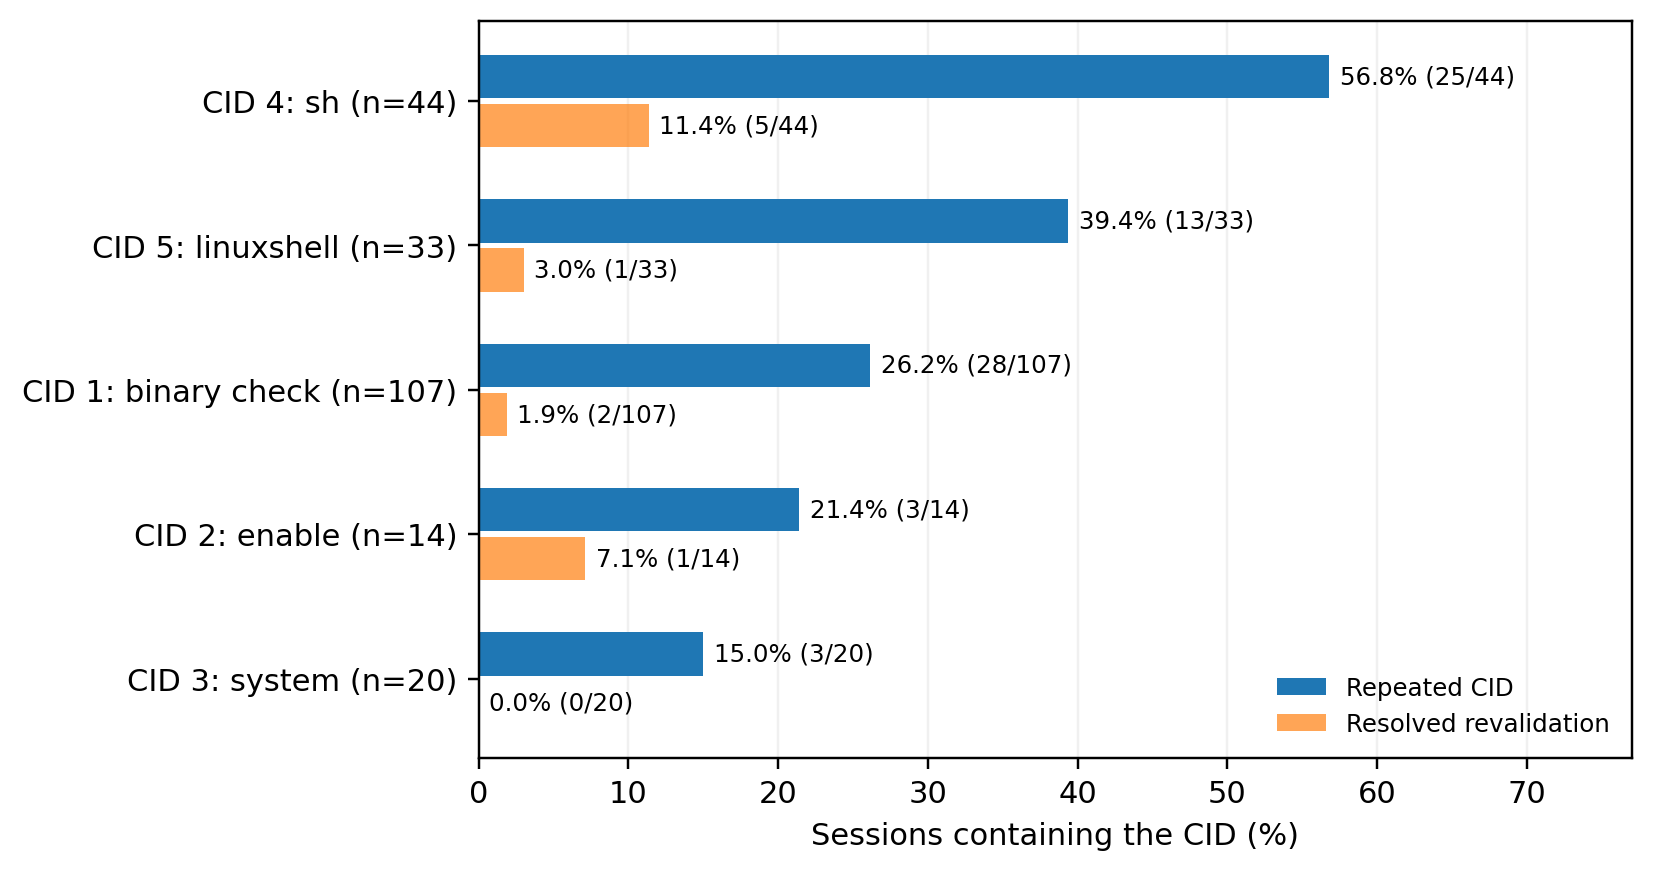
\includegraphics[width=\linewidth]{images/fig_cid_revalidation_verified.png}
 \caption{Repeated CIDs versus timestamp-resolved revalidation.}
\end{subfigure}
\caption{Audited empirical properties of the observed SSH traces:
(a) distribution of recorded-event depth, (b) continuation only when a
later mapped input has a strictly greater timestamp than the earliest
relevant probe, and (c) repeated commands distinguished from
revalidation with a timestamp-resolved intervening different command.
Panel (b) uses the fixed CID groups documented with the analysis code;
proportions are descriptive and not response-effect estimates.}
\label{fig:ssh_empirical_motivation}
\end{figure*}

These observations motivate the subsequent formulation in two ways.
First, protocol-visible properties such as shell availability, device
interface behavior, and filesystem or binary characteristics can be
queried repeatedly within a session. A response-selection mechanism
should therefore preserve consistency with accumulated EFSM state,
unless a valid modeled state transition changes the property. Second,
observed continuation differs across command contexts, which motivates
investigating whether response adaptation can be localized rather than
introduced indiscriminately. Crucially, the present event-and-command
logs contain no response-conditioned outcome comparison and cannot
establish that alternative honeypot responses cause different attacker
continuations. The KDP analysis must separately identify interaction
conditions where historical alternative responses are associated with
sufficiently supported differences in subsequent behavior. The
formulation that follows consequently distinguishes EFSM-constrained
response admissibility from response-sensitive decision localization.
